\documentclass[a4paper, 12pt, titlepage]{article}

% Including needed packages
\usepackage[margin=2cm]{geometry}
\usepackage{amsmath}
\usepackage{amssymb}
\usepackage{amsthm}
\usepackage{graphicx}
\usepackage{subfig}
\usepackage{float}
\usepackage{pgf}
\usepackage{tikz}
\usepackage{dsfont}

\newcommand{\norm}[1]{\lVert#1\rVert}
\usetikzlibrary{automata,positioning}

\title
{{\em Machine learning 2}\\
Exercise sheet 10}
\author{FLEISCHMANN Kay, Matrnr: 352247\\
	ROHRMANN Till, Matrnr: 343756}
\date{\today}

\begin{document}

\maketitle
\section*{Hidden Markov Model}

Let $A_{i,j}$ the transition matrix between hidden states $x_i$ and $x_j$. $B_{i,j}$ is the the probability, beeing in state $x_i$ to observe $y_j$.
The following matrices $A$ and $B$ describe two hidden states and two possible observations.

\[
A= 
 \begin{pmatrix}
  0.1 & 0.9 \\
  0.5 & 0.5
 \end{pmatrix}
\]

\[
B=
 \begin{pmatrix}
  0.2 & 0.8 \\
  0.4 & 0.6
 \end{pmatrix}
\]

\subsection*{19.a Implementation of Viterbi algorithm}
\subsection*{19.b Experiment results}

Perform the following experiment: for the Hidden Markov Model of sheet 9, that is, generate sequences of length $l= 5, 10$ and $20;$ for each length generate a number of $N = 1000$ pairs of output sequences and hidden state sequences. On these sequences, for each length , compare $(i)$ the Viterbi algorithm and $(ii)$ the algorithm which randomly uniformly estimates a state sequence by (i) plotting for each length , and all integers $1 \le k \le l$ , the relative frequency of the algorithm correctly estimating the hidden state at position $k$ (this is three plots, one for each , and in each plot two curves), and $(ii)$ for each length , computing the relative frequency of both algorithms succeeding in completely identifying the state sequence correctly (this is two numbers for each of the three ).

\begin{figure}[h]
	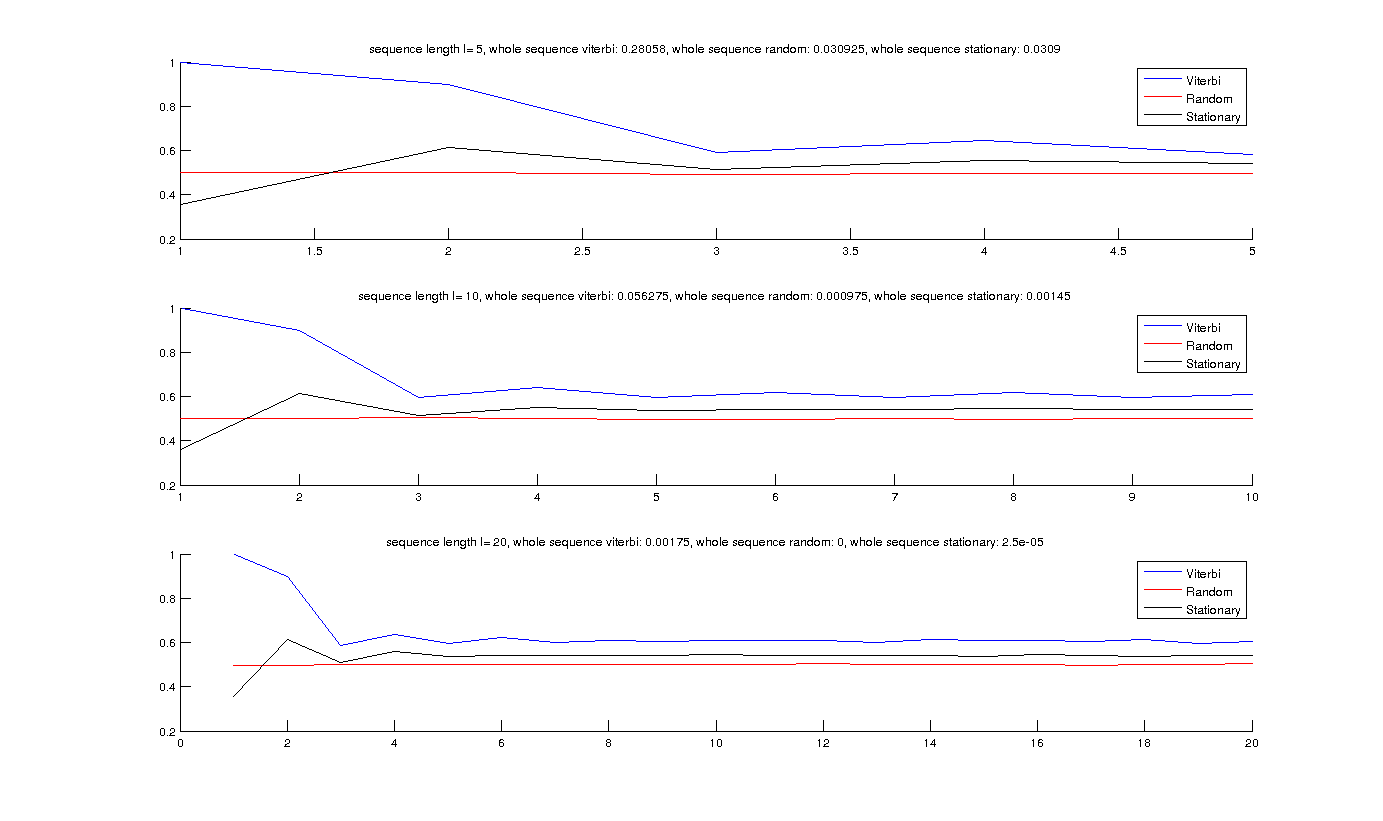
\includegraphics[width=\textwidth]{images/experiment_results.png}
	\caption{This plot compare the viterbi results with the funktion which randomly generate the hidden states. The plot shows the relative correct detected hidden states with diffrent settings in the experiment. }
\end{figure}


\end{document}